\label{chap:4}

A naive approach to SRAM PUFs would be to choose a random selection of cells among the available cells. As pointed out in section \ref{sec:HDAs}, this would leave all the work to the ECC step and would come at a prohibitive cost considering the limited reliability of standard SRAM PUFs responses. There are a variety of criteria to choose the best cells in a SRAM. An ideal selection would improve the reliability of the response without being detrimental to uniqueness or uniformity. These cells should also provide a better response under the worst corners of performance, not just under nominal conditions. 

In this chapter, some commonly used prevalent bit selection techniques are discussed. They serve as reference to compare the new bit selection technique, Maximum Trip Supply Voltage (MTSV), that tries to improve the existing techniques. Afterwards, this new technique is presented and validated with experimental data.

\section{Multiple Evaluation}
\label{sec:ME}
In Multiple Evaluation (ME) several power-up evaluations are performed on each cell, either to elaborate a response by majority vote \cite{Bhargava2012}, or to discard those cells that do not always power-up to a given value \cite{Baturone2015}. A key aspect of this method is that a fixed number of measurements must be selected: for instance, 20 measurements were chosen as a good trade-off in \cite{Baturone2015}. However, it is also shown in \cite{Baturone2015} that many cells that returned the same value for the first 20 power-ups, returned at least one “erroneous” value (i.e., their nonpreferred value) in the next 60 measurements, since 80 power-ups were performed to each cell. This is illustrated in fig. \ref{fig:unstable_me} for one of the chips used later in this work. In \cite{Bhargava2012}, no specific number of evaluations is set; however, the necessity of making this choice is clearly stated and the possibility of using from 10 to 100 evaluations is mentioned. Nevertheless, the appropriate number of evaluations depends on several factors, such as the technology node. Choosing well would thus require a tedious experimental study. In fact, this type of multiple evaluation may require a prohibitively high number of power-ups, thus delaying an on-line response, and significant hardware resources \cite{Liu2017}. 

\begin{figure}[H]
    \centering
    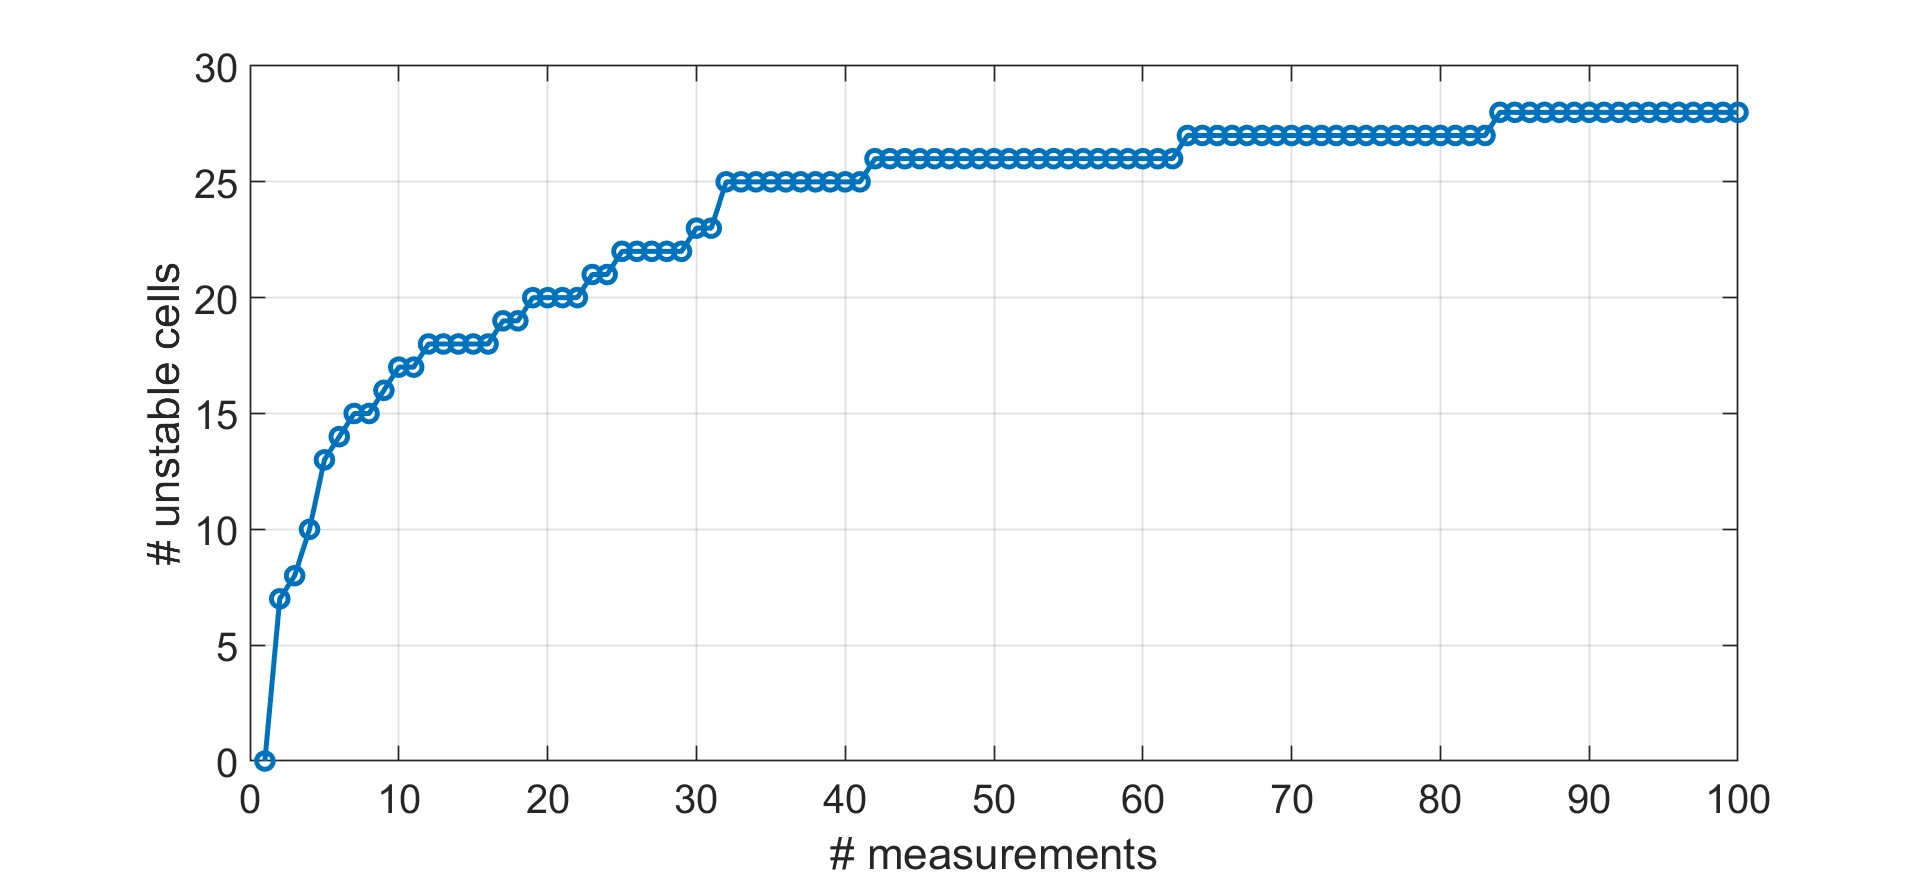
\includegraphics[width=16.5cm]{images/unstalbe_me.jpg}
    \caption{Number of unstable SRAM cells with respect to the number of power-ups for one of the chips. }
    \label{fig:unstable_me}
\end{figure}

\section{Data remanence}

The technique presented in \cite{Liu2017} consists of two remanence tests: writing ‘1’ (or ‘0’) to the entire SRAM cell array and shutting down the power supply for a short time interval until a few cells flip. The technique exploits the fact that the cells that flip with shorter power-off durations have the strongest tendency towards the value that has not been written. This methodology has proven to be effective for experiments performed under different temperatures and power ramp times, and under device aging \cite{Liu2017}. This approach has been tested in a design fabricated in an ultra-low leakage technology, which requires relatively long power-down times (in the order of hundreds of milliseconds) to observe those bit flips. However, much shorter data remanence times are expected for SRAMs built in advanced CMOS technologies (e.g., below microseconds \cite{Liu2017}), which may turn this technique impractical to use on certain technologies. If power-on and power-off times in the order of microseconds have to be precisely controlled, it is clear that the ramp rates must be much faster than that. However, in \cite{Wang2018}, it is shown that the power-up states are especially sensitive to such factors like noise when ramp rates in the range of nanoseconds to microseconds are used. An option to overcome this issue is to operate these tests at low temperatures, at which longer remanence times are expected \cite{Anagnostopoulos2018}. To this end, temperatures of tens of degrees Celsius below zero are necessary, which usually involve the utilization of liquid nitrogen as cooling method. This makes the method further unfeasible for practical applications. Moreover, to control the power-on and power-off times precisely, an additional microcontroller must be used. Therefore, this solution is not suitable for applications with resource-constrained devices.


\section{Exploting the Power Supply Ramp Rate}
\label{sec:bitselection:supply_ramp}
In \cite{Wang2018}, a method to calibrate the strength of the SRAM cells is presented. Its authors claim that, if the SRAM is turned on by ramping the $V_{DD}$ node from low to high at a rapid rate, the power-up of individual cells is decided entirely by the threshold voltage mismatch in the PMOS transistors in each cell. On the other hand, if the SRAM is powered up by rapidly ramping the $V_{SS}$ node from high to low, the power-up state of each cell will depend on the threshold voltage mismatch between the NMOS transistors in the cell. Otherwise, if a slow ramp is used (‘over several seconds’ in \cite{Wang2018}), both NMOS and PMOS pairs play a role in determining the state stored on the cell after the power-up.


From that theoretical starting point, the following method is proposed to identify the strongest cells: first, a fast $V_{DD}$ ramp test is performed to investigate the preferred power-up state of each cell as determined only by its pair of PMOS core transistors. Then, an equivalent test is performed, this time ramping down the $V_{SS}$ -node from high to low, to identify the preferred power-up state as determined only by its pair of NMOS core transistors. Considering both the preferences of the PMOS and NMOS transistors separately, there are four possible combinations (‘0,0’, ‘0,1’, ‘1,0’, ‘1,1’). Thus, around 50\% of the cells are expected to power-up to the same state in both tests. By selecting these, a set of cells where both the NMOS and the PMOS transistor pairs individually bias the cell to the same power-up state is obtained. Finally, the strength of that set of cells is quantitatively calibrated. For that, the SRAM is written with a logic ‘1’ (or ‘0’) and then $V_{DD}$ is slowly ramped down to a small voltage (e.g., 0.1V).

Then $V_{DD}$ is ramped back again to its nominal value. This process is repeated while varying the lower limit of the supply voltage (e.g., 0.1V, 0.11V, 0.12V, etc.). If the initially written value was ‘1’, cells that have ‘0’ as their preferred value may flip to ‘0’ during the above described process. While cells with a stronger tendency towards ‘0’ may already flip their value at higher values of the decreased $V_{DD}$ (e.g., 0.2V), cells with a weaker tendency will need a lower $V_{DD}$ to flip their value (e.g., 0.1V).

However, there are some limitations to this technique. First, unlike other conventional methods to calibrate the strength of SRAM cells \cite{Bhargava2012,Baturone2015,Liu2017}, it requires the realization of ramps in two different nodes of the SRAM cell $(V_{DD} \ \mathrm{and} \ V_{SS} )$. Second, it requires the utilization of two types of ramps, slow and fast, with ramping rates orders of magnitude apart. This translates into additional hardware resources if the method is to be implemented on-chip. Moreover, the utilization of fast ramps at both supply nodes is counterproductive. While fast ramps are performed in 1 nanosecond in the work presented in \cite{Wang2018}, it is also stated in that work that power-ups performed at such fast ramps are very sensitive to factors such as noise or device degradation. Therefore, the classification performed to select the potential candidates using ramps in the nanosecond scale may be incorrect. Finally, no silicon experimental results that validate the method under real operating conditions are presented in \cite{Wang2018}: only simulation results using a Predictive Technology Model (PTM) for a 32-nm bulk technology, with estimated variability parameters, are provided. Moreover, background noise, supply voltage variations, circuit noise, temperature variations or circuit degradation due to aging effects were not considered, even though these are known to be critical factors in the performance of SRAM-based PUFs. 


% Other works that follow a similar approach and their results. 1-2 Pages

% To investigate the effect that a limited number of evaluations has on the determination of the cell strength, a simple Multiple Evaluation test has been performed with the experimental setup used in this work (see Section IV). Figure 2 shows the number of unstable cells with respect to the number of performed evaluations for one of the chips. A similar behavior has been found for all measured chips.

% Considering five different samples of the same chip containing 832 SRAM cells each, the average number of unstable cells after 10 evaluations is 15, while this number increases to 26 after 100 evaluations. Therefore, a reduced number of evaluations will detect only a portion of the unstable cells.

% From the outcome of this test, it becomes clear that a number of evaluations in the order of the ones proposed in [6] or [7] would lead to label some cells as “strong” when in fact these present a relatively high probability of powering-up to their non-preferred value.

% There is another limitation of this method that should be addressed. As it will be shown in Section V, fresh cells (i.e., not aged) that always return the same value when poweredup, may lose their stability after circuit aging, or in the presence of temperature and/or supply voltage variations.

% This fact makes the Multiple Evaluation method unable to find SRAM cells that are truly resilient to these phenomena and, therefore, not suitable for creating a PUF instance.

\section{Maximum Trip Supply Voltage (MTSV) method}
\label{sec:MTSV}
A new bit selection technique is now described. First, a description on how it works is provided. This technique is then tested experimentally against the most popular one available, multiple evaluation. The experimental setup used for these tests is described, and then the results are presented. 


%Detailed description of MTSV. 2-3 Pages.
\subsection{Description}

To overcome some of the limitations that the above-discussed methods present, a new approach is described in this section. The idea behind this method, which will be referred here as MTSV method, is to evaluate the strength of a cell by writing its non-preferred value on it, then lowering $V_{DD}$ for a given period of time, raising it again and checking if the cell has changed its value.

 For the sake of illustration, two cells, \textit{cell1} and \textit{cell2}, which tend to go to ‘0’ but with different strength, will be considered. A ‘1’ is written in both cells and then $V_{DD}$ is lowered and then raised (to its nominal value) repeatedly (with $V_{DD}$ dropping to a lower value with each repetition) until the cell flips its power-up value to ‘0’. It is found that \textit{cell1} flips at $V_{DD1}$ while \textit{cell2} does it at $V_{DD2}$. \textit{Cell1} is said to have a stronger tendency to the ‘0’ state if $V_{DD1}>V_{DD2}$. Therefore, the idea is to classify all the cells in an SRAM by writing their least-preferred value on them, lowering their supply voltage to different values, and recording at which voltage value each cell starts flipping to its preferred value. This voltage value is their data retention voltage (DRV); strongest cells will thus be those with a higher DRV. Cells that, while lowering their $V_{DD}$ at different values during the MTSV procedure, show a random behavior, for example returning ‘0’ and ‘1’ alternatively at different values of decreased power supply, do not have a strong power-up tendency. Therefore, they are labelled as unstable, no DRV value is assigned to them and do not even enter the power-up strength classification procedure.

While the Multiple Evaluation methodology introduced in the previous section may require a prohibitively high number of evaluations, the technique used in this work, on the other hand, requires a much lower number of iterations. For instance, if the range of supply voltages within which the cells experience a bit flip is bounded between ~\SI{80}{mV} and ~\SI{280}{mV} (as it is the case of this work), and assuming a step size of \SI{10}{mV} for the evaluation, a total number of 21 steps is needed. Additionally, unlike \cite{Liu2017}, no precise timing of the power-off and power-on durations is needed, which becomes especially critical when these are in the range of nanoseconds to microseconds. Finally, unlike the method in \cite{Wang2018}, only one type of ramp in one of the nodes is needed. This is important in different aspects. First, only ramps at the SRAM $V_{DD}$ node are performed (no ramp at the $V_{SS}$ node is required). Second, only one ramp rate is needed, while in \cite{Wang2018} two different ramp rates that are orders of magnitude apart were needed.

Furthermore, the ramp used in this work is in the order of a few milliseconds, which results in a reproducible PUF response, while the method in \cite{Wang2018} used fast ramps in the range of nanoseconds, thus producing PUF responses that are very sensitive to factors such as noise or device aging. Finally, by not selecting the candidate cells only among those where both PMOS and NMOS transistor pairs produce a bias towards the same power-up state, potentially stable cells are not discarded, as it occurs in \cite{Wang2018}.



\subsection{Chip}
\label{sec:chip}
The circuit used in this work is an array of 832 SRAM cells, a photograph of which is depicted in Figure \ref{fig:KIPTsram} \cite{Saraza-Canflanca2018}. These cells are distributed in 32 rows by 26 columns. The 6T SRAM cells have been sized with W = \SI{80}{nm} and L = \SI{60}{nm} for the access transistors and the PMOS pull-up transistors, and W = \SI{160}{nm} and L = \SI{60}{nm} for the NMOS pull-down transistors, following conventional sizing criteria. The chip has been designed so that individual access and control of every terminal of each SRAM cell is granted, as shown in fig. \ref{fig:KIPTsramcell}. This is necessary to properly perform the different tests on each SRAM cell, including normal operation tests, aging tests or simply switching off the cells. 

\begin{figure}[H]
    \centering
    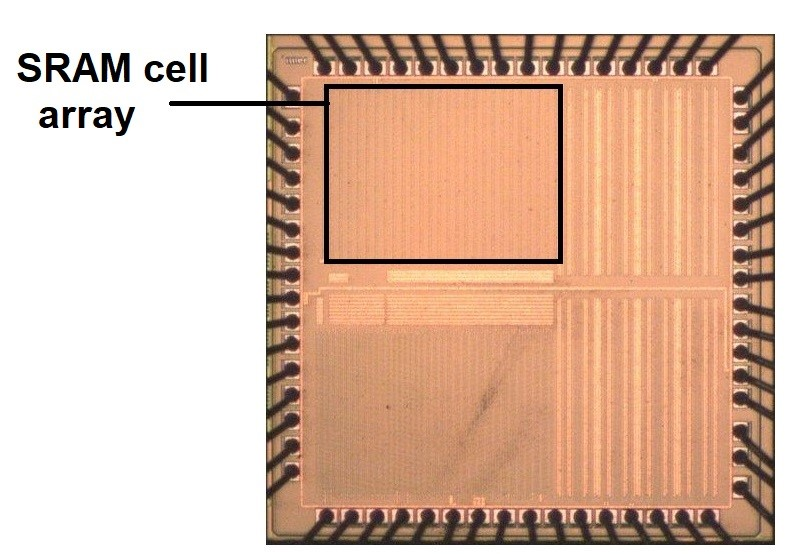
\includegraphics[width=10cm]{images/KIPTsram.jpg}
    \caption{Photograph of the chip used in this work, with the part corresponding to the array of SRAM cells highlighted.}
    \label{fig:KIPTsram}
\end{figure}

For the aging tests, as the degradation of the SRAM operation will extend along years, physical characterization is not possible under normal operation conditions. Therefore, accelerated aging conditions, e.g., by using higher operating voltages on SRAM terminals and/or higher operating temperatures, are applied during certain periods of time, in the range of seconds to hours. Some SRAM figure-of-merit must be measured before and after the stress cycle to compute its degradation.

\begin{figure}[H]
    \centering
    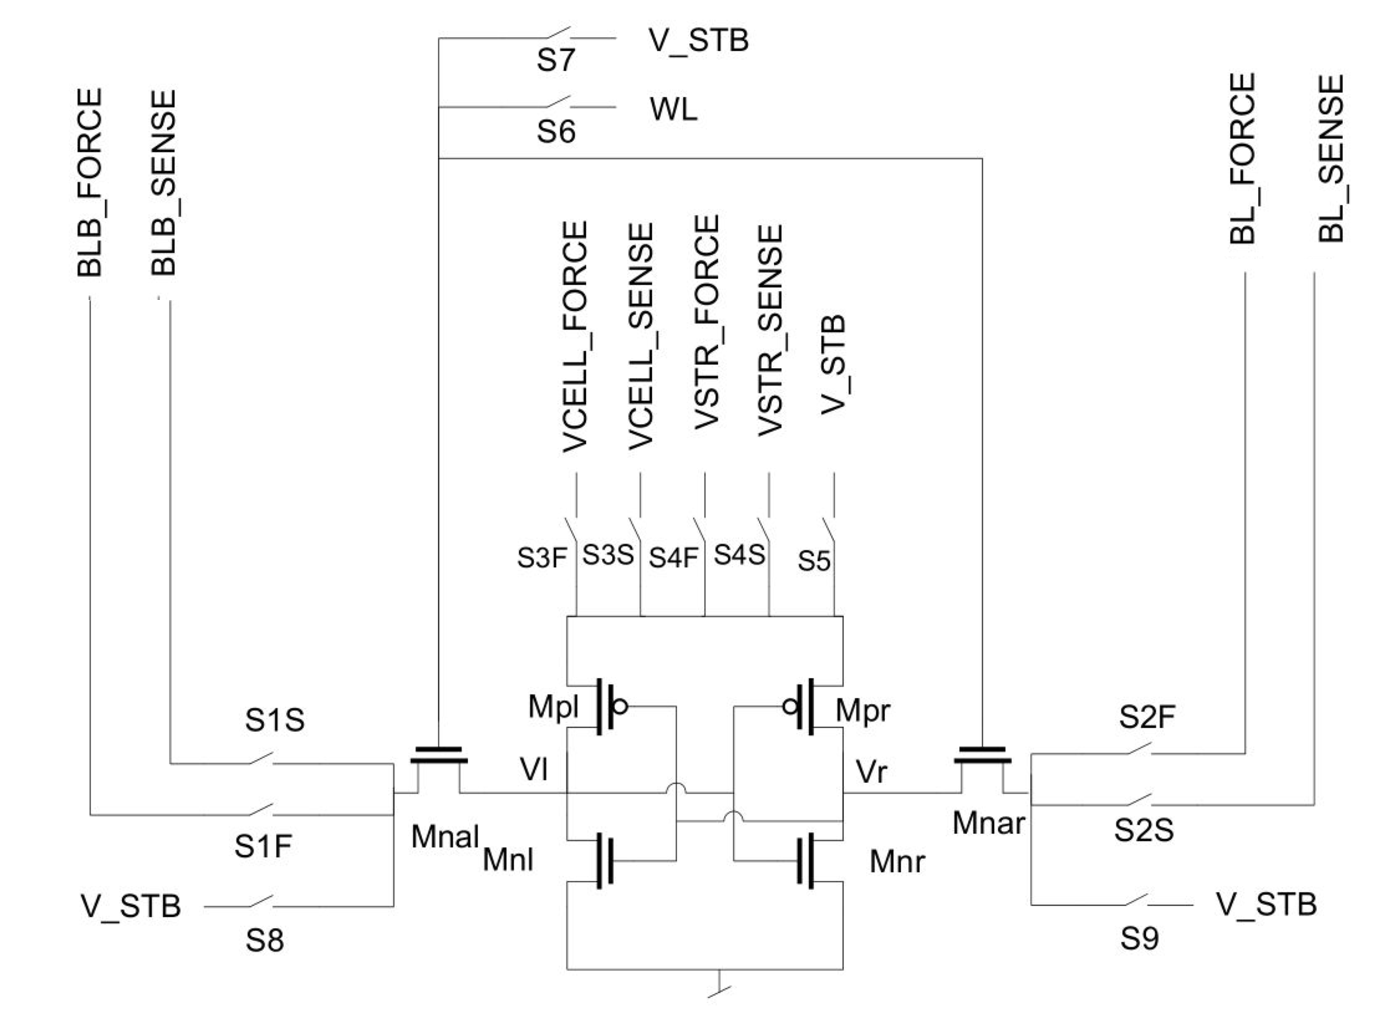
\includegraphics[width=10cm]{images/KIPT cell modified.pdf}
    \caption{SRAM cell with transmission gates for appropriate terminal
access and control.}
    \label{fig:KIPTsramcell}
\end{figure}



It must be noticed that, as explained in section \ref{sec:aging}, in some aging phenomena, e.g., BTI, the stressed devices start recovering their original electrical parameters, once the stressed condition is removed. Therefore, accurate timing of stress and measurement stages must be established. Because of the stochastic nature of aging phenomena, stress and characterization tests must be performed over a large number of devices. The fact that a large number of cells have to be stressed during relatively long times implies a characterization bottleneck if the process is performed serially, cell by cell, especially if the recovery period has to be measured since cells are read-out serially. For this reason, each cell included digital control circuitry that allows parallelization of stress of several cells, while read-out of another cell is performed, strongly reducing the time of these experiments. As an example, if accelerated aging conditions are applied for 10,000 s, it would take around 97 days to characterize all 832 cells serially and around 28 hours to do so parallelly.

Force and Sense (F\&S) techniques are needed for accurate measurements. Therefore, independent F\&S paths are required to access those terminals where current is flowing and a voltage drop can occur.
 
The array includes row and column decoders to individually select each SRAM cell. Digital control circuitry is included in each cell as well as access circuitry (transmission gates, TG) that connect each terminal of each cell to output pads, as shown in Figure 4.3. Four control bits are used to control the TG´s at each node of the SRAM cell, defining 4 different operation modes for each cell: 

\begin{enumerate}
    \item \textbf{Measure mode:} This operation mode has been designed to connect the word line and bit line terminals to the word-line and bit-line analog paths, respectively, and the cell power supply terminal to the standard power supply path. In this operation mode, the selected cell can undergo any write or read operation, or hold some data. Voltages can be fully controlled so that any SRAM figure-of-merit can be properly measured.
    \item \textbf{Stress hold mode:} This operation mode has been designed to connect the power supply terminal of the SRAM to the stress power supply path. As shown in Fig. 3, this path is independent of the standard power supply. This feature enables the parallelization of the stress hold mode of one SRAM cell together with other operations in other cells.
    \item \textbf{Stress AC mode:} This mode has been designed to perform write or read operation under stress conditions, up to 3.3V, applied to the word line, bit lines and power supply terminals.
    \item \textbf{Stand-by mode:} This operation mode connects bit line, word line and power supply terminals to the stand-by analog paths (VSB). This operation mode has been designed to keep all cell terminals at 0V, and therefore under no aging process.
\end{enumerate}



While this modified SRAM cell allows for accurate accelerated aging tests, its characteristics are not different in any way from the standard 6T SRAM cell considered in chapter \ref{chap:3}. The experimental data and conclusions obtained from it can be generalized for a generic SRAM PUF. The MTSV technique itself does not need this particular design. Further information about the circuit design can be found in \cite{Saraza-Canflanca2018}.

\subsection{Experimental setup}
\label{sec:exp_setup}
The main components of the experimental setup used in this work are depicted in Figure \ref{fig:expsetup}. A full-custom Printed Circuit Board (PCB) has been used for the different tests, together with a power supply generator for the biasing of the PCB and the chip. A Keysight B1500 semiconductor parameter analyzer equipped with 4 High Resolution Sense Measurement Units (HRSMU) has been used for voltage application and measurement. The HRSMUs have a F\&S system that, together with the F\&S connection implemented in the circuit, allows the accurate application of voltages by avoiding undesirable voltage drops in the chip. The temperature tests have been performed using an ACS climatic chamber, which allows the stable and homogeneous application of temperature on the chip.

\begin{figure}[t]
    \centering
    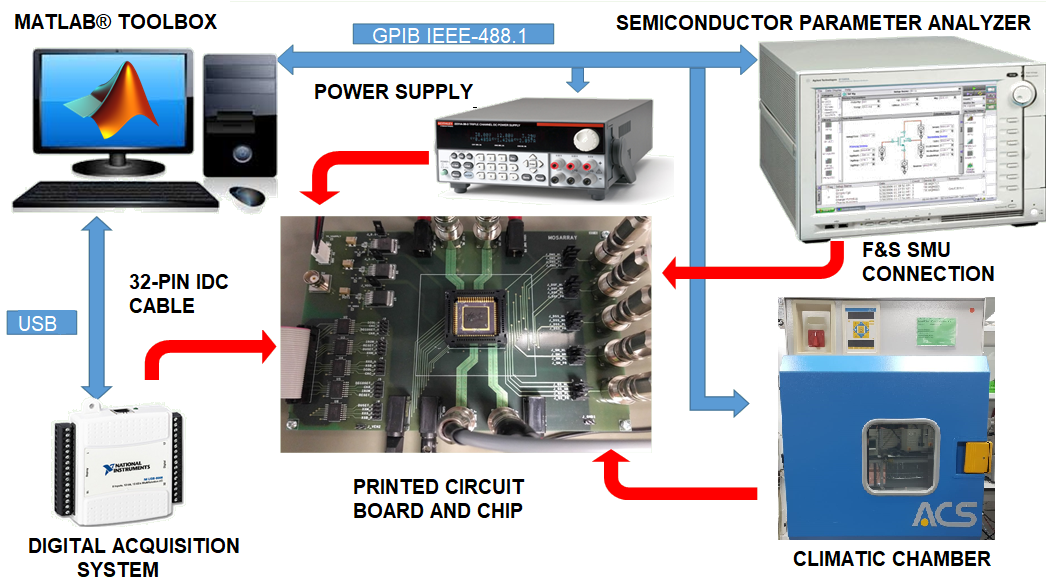
\includegraphics[width=14cm]{images/experimental_setup.png}
    \caption{Representation of the experimental setup used in this work.}
    \label{fig:expsetup}
\end{figure}

\subsection{MTSV experimental performance}

The adequacy of the MTSV method has been tested under four different scenarios: at nominal conditions, after the circuit has been subject to accelerated aging, under temperature variations, and under supply voltage variations. The metrics used to evaluate the quality of the responses are the ones presented in sec. \ref{sec:Metrics}. The values obtained without performing bit selection are the reference point to assess the effectiveness of ME and MTSV. The ramps used in this work are in the order of a few milliseconds, where the power-up state is expected to be scarcely impacted by factors such as noise \cite{Wang2018}. 

\subsubsection{Nominal conditions}

The first step is to measure the response of the chip under nominal conditions of temperature and supply voltage. Five different chips are used during these measurements to ensure that the results are valid under inter-chip variations. Since the inter hamming distance is measured across all chips, it is a good starting point. The result is obtained using eq. \ref{eq:interhd}:

\begin{equation}
\text{mean}_\text{InterHD}=49.9398 \%
\end{equation}

This result is good, close to the ideal 50\%. It confirms that there is no relevant correlation between the power-up behavior of different chips’ cells, and therefore uniqueness is expected from the different PUFs’ responses.

The next step is to classify the cells in terms of their power-up response following the MTSV method. Figure \ref{fig:mtsvflow} shows a flow diagram of how the classification of each cell is done, according to its power-up strength: first, its non-preferred power-up value was written on it. Then, its supply voltage was decreased to different values ranging from $\SI{280}{mV}$ to $\SI{80}{mV}$ and the content of the cell was read at each step. Cells that showed a random behavior, for example returning ‘0’ and ‘1’ alternatively at different values of decreased power supply, were labelled as “unstable”. Among the five chips, the number of unstable cells ranged between 40 and 50 out of the 832 cells of each chip. Interestingly, these cells correspond roughly to the cells labelled as unstable by the Multiple Evaluation method when a large enough number of power-ups is performed (see Figure \ref{fig:unstable_me}). Therefore, cells that did not show a random behavior during the MTSV procedure, that is, cells that flipped their content for one given VDD (their DRV value) and continued flipping their content for any VDD below their DRV value, correspond to the cells labelled as completely stable (0\% erroneous power-ups) by the Multiple Evaluation procedure. These cells were assigned that DRV value and were ordered from strongest (highest DRV value) to weakest (lowest DRV value). Note that the Multiple Evaluation method is not able to perform this classification to the cells it labelled as stable, since they all powered up to the same value at each evaluation. 


\begin{figure}[H]
    \centering
    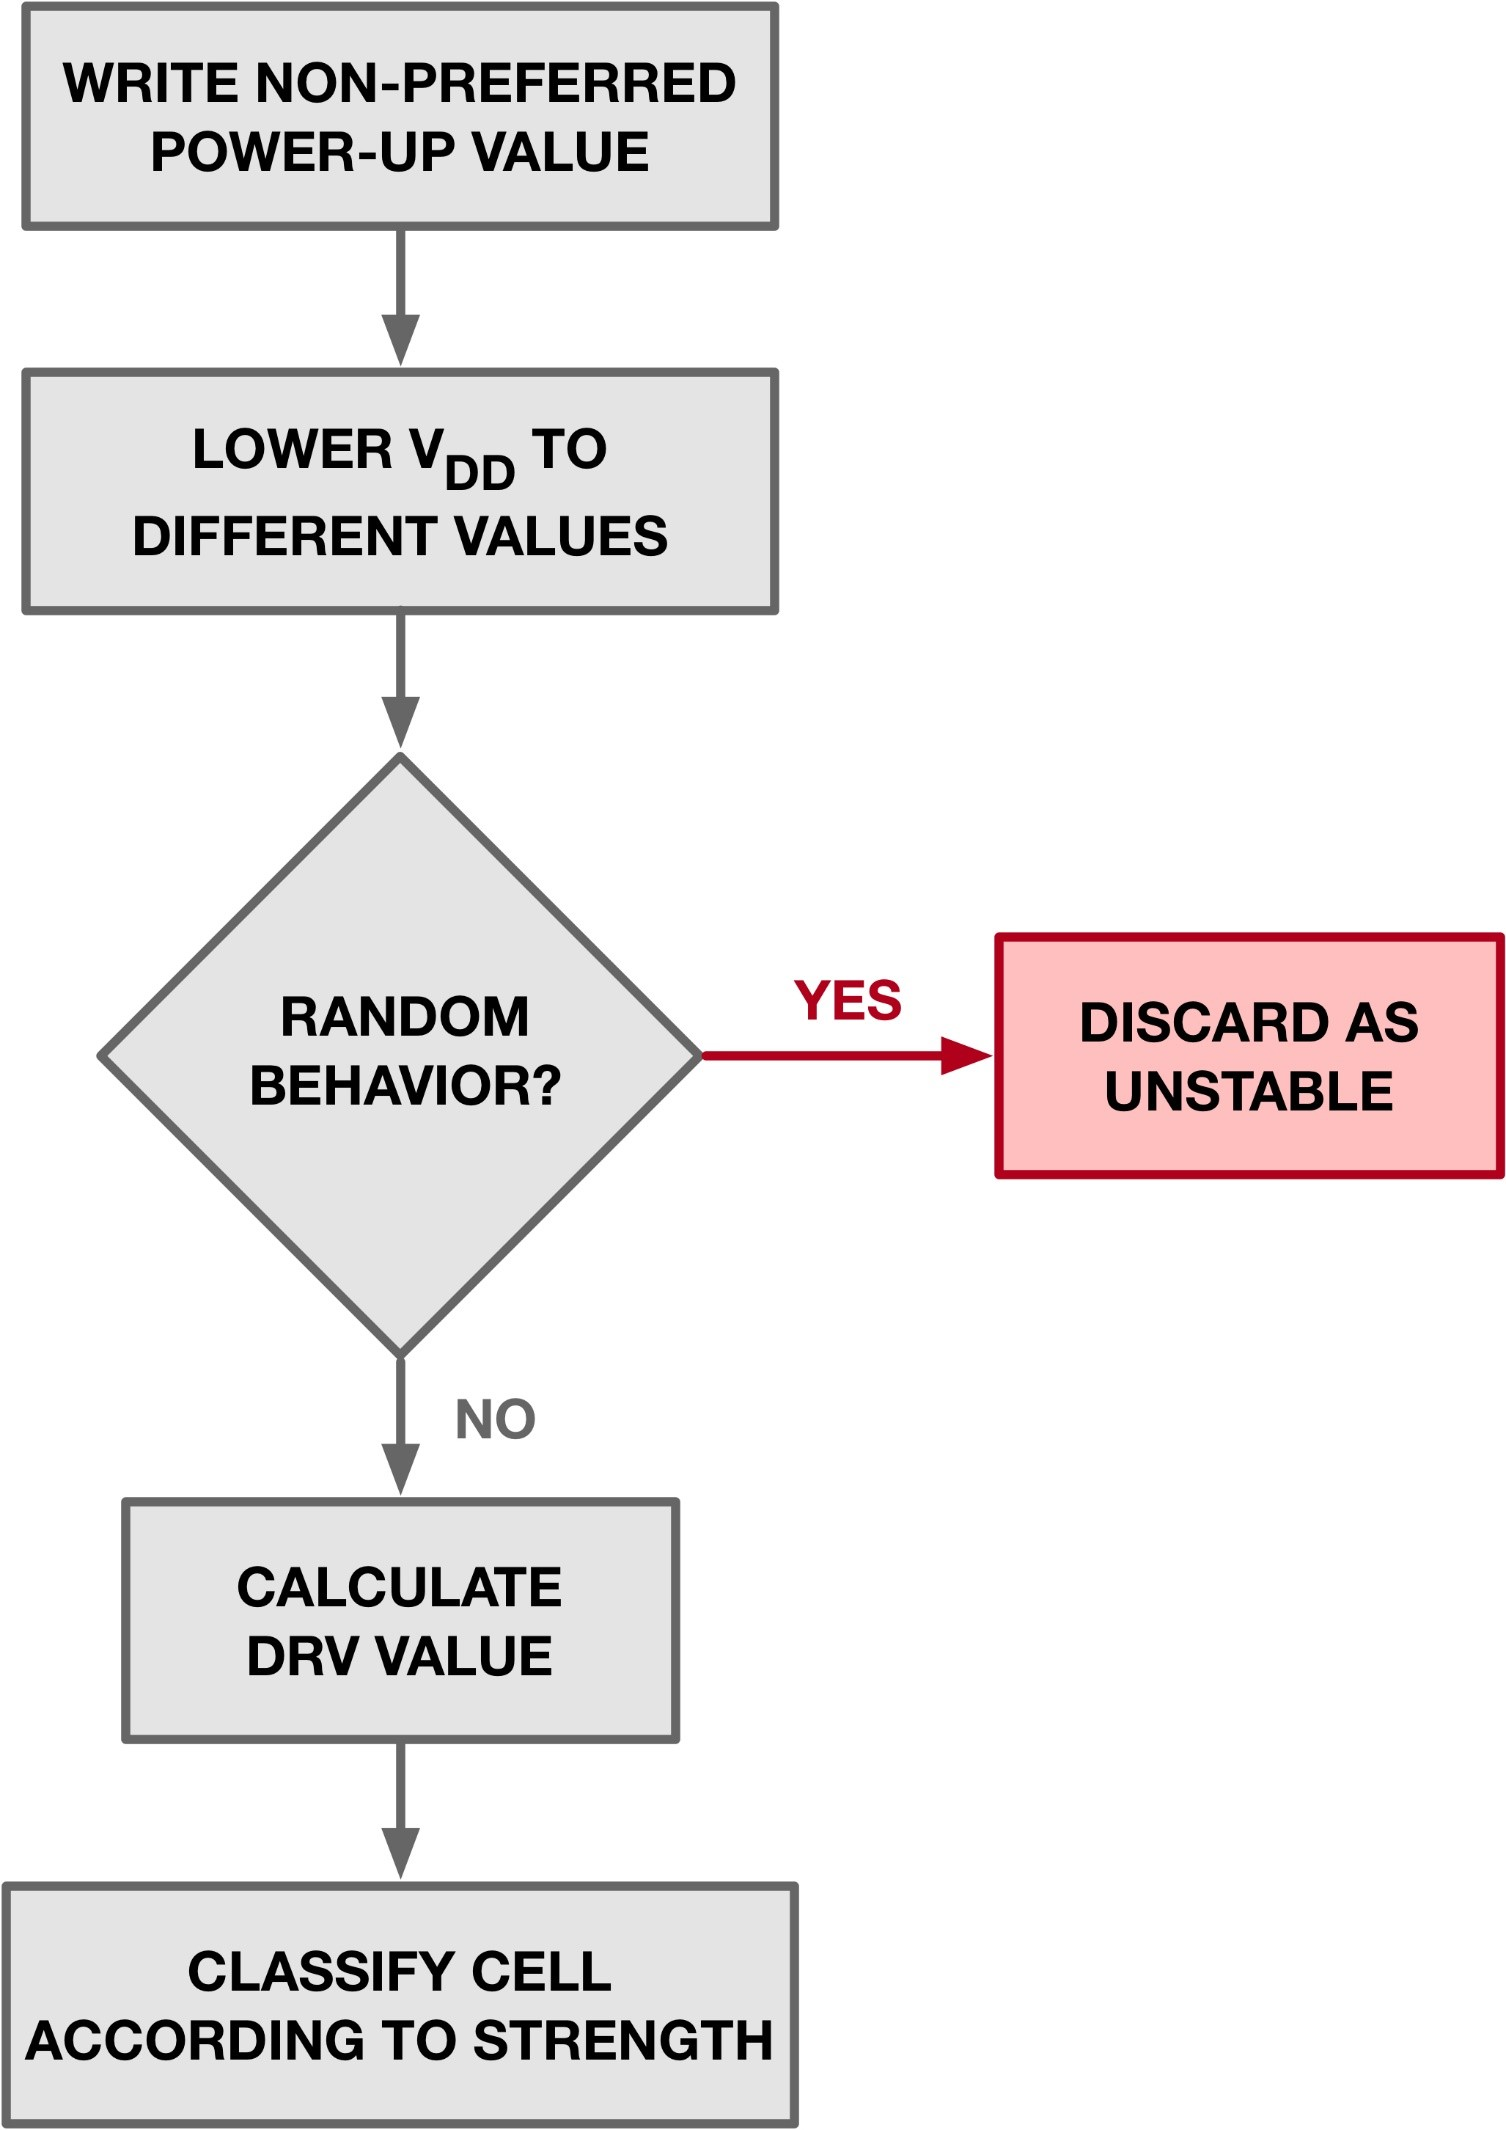
\includegraphics[width=6cm]{images/mtsvflow.jpg}
    \caption{Flow diagram of the procedure used to classify each cell according to its power-up strength. }
    \label{fig:mtsvflow}
\end{figure}

% By the ME approach, cells are labelled as unstable if they do not always return the same value after powering up. The number of unstable cells will increase as more power-ups are performed. Among the five chips the average number of unstable cells after 10 evaluations is 15, while this number increases to 26 after 100 evaluations. Accordingly, a reduced number of evaluations will detect only a portion of the unstable cells, as shown in fig.\ref{fig:unstable_me}. These cells correspond roughly to the cells labelled as unstable by the Multiple Evaluation method when a large enough number of power-ups is performed. Therefore, cells that did not show a random behavior during the MTSV procedure, that is, cells that flipped their content for one given $V_{DD}$ (their DRV value) and continued flipping their content for any $V_{DD}$ below their DRV value, correspond roughly to the cells labelled as completely stable (0\% erroneous power-ups) by the Multiple Evaluation procedure. These cells were assigned that DRV value and were ordered from strongest (highest DRV value) to weakest (lowest DRV value). Note that the Multiple Evaluation method is not able to perform this classification to the cells it labelled as stable, since they all powered up to the same value at each evaluation. Naturally, if no bit selection technique is used the unstable cells are included in the pool of available cells which significantly worsens the quality of the response. 

In order to evaluate the method, the 50 strongest and the 50 weakest cells of each chip were selected, so that their strength could be compared between them and also to the rest of the array. In the following, “weakest cells” refers to the weakest cells among the ones that were not labelled as “unstable” during this first phase of the MTSV procedure. 

It must be noted here that selecting 50 cells has been an arbitrary decision, since a larger or a smaller selection would serve as well for the purpose of this experimental validation. The goal here is not to create a specific PUF instance, but to prove that the MTSV method allows the selection of the strongest and more robust SRAM cells.

Figure \ref{fig:DRVhist} shows a histogram of the DRV values for the SRAM cells that display a tendency to power-up to one of the possible values. The histogram corresponds to an MTSV experiment with $V_{DD}$ step size of \SI{5}{mV}, performed on 832 cells of one of the chips. The strongest cells correspond to the right tail of the histogram, i.e., those with a higher DRV value, while the weakest cells correspond to the left tail of the histogram. Unstable cells do not appear in the histogram, since no DRV value could be assigned to them.

\begin{figure}[t!]
    \centering
    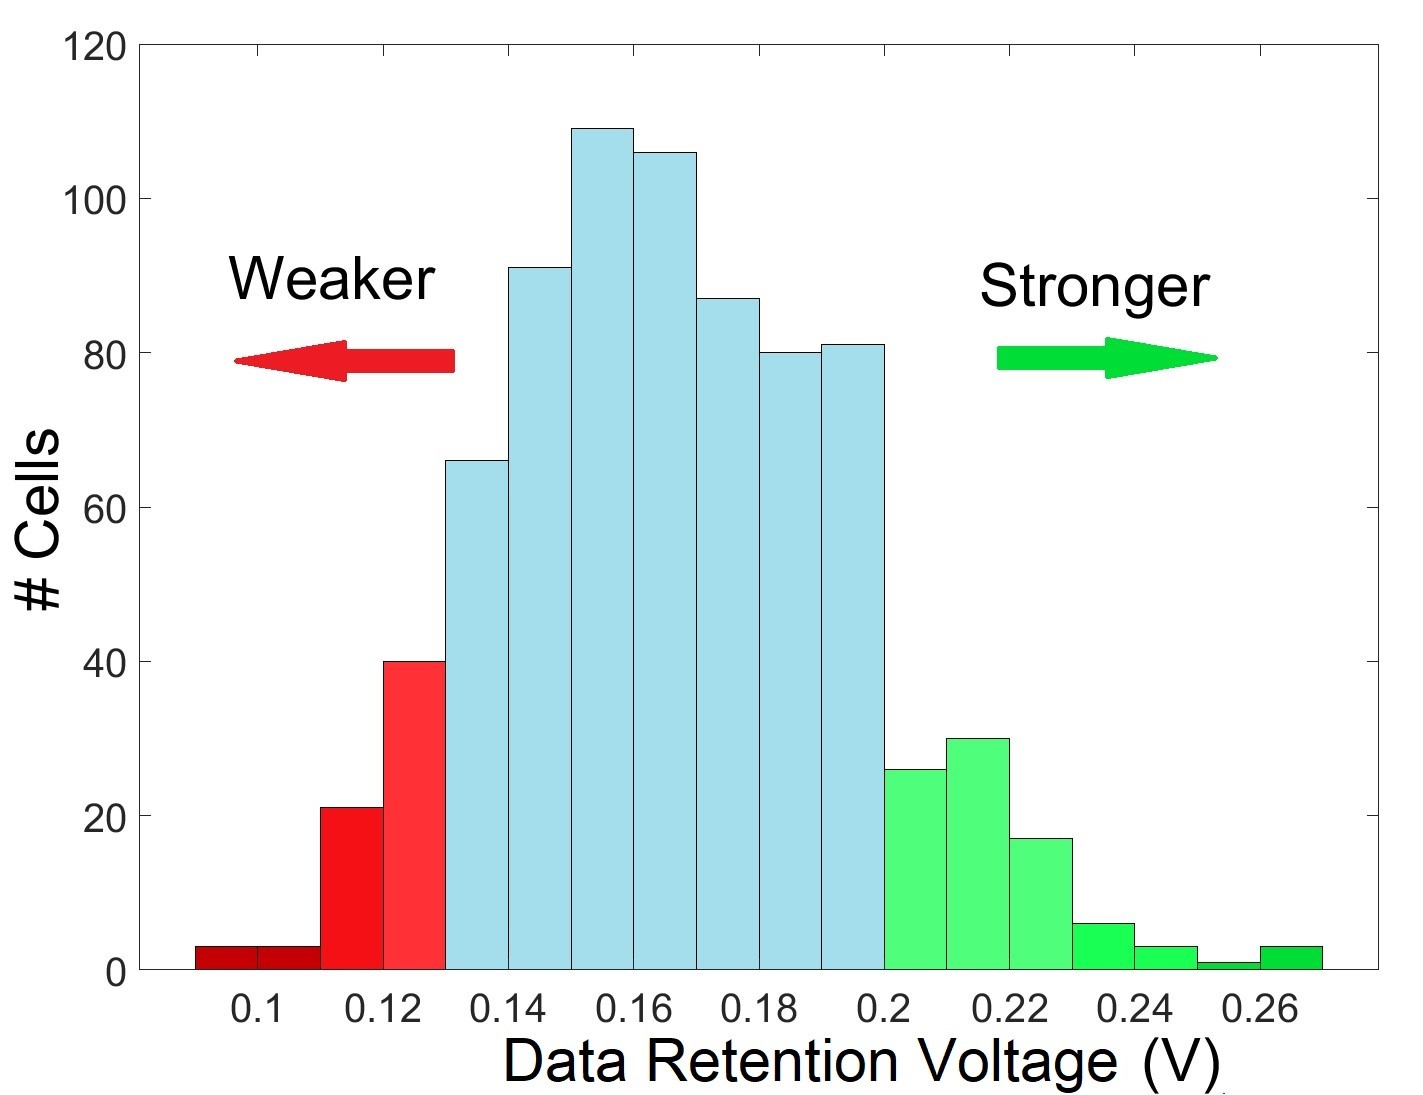
\includegraphics[width=12cm]{images/DRV histogram.jpg}
    \caption{Histogram of the $V_{DD}$ values at which cells (in one of the chips) start flipping from their non-favorite to their favorite value. }
    \label{fig:DRVhist}
\end{figure}


Then, to evaluate the adequacy of the MTSV-based classification, 2,500 power-up evaluations are performed for the 50 strongest and the 50 weakest cells of each chip, and 200 power-ups for the rest of cells. The number of power-ups applied to the strongest and weakest cells is higher than the one commonly used in the Multiple Evaluation method, but for the purpose of the comparison made here, this number will provide a much more precise evaluation of the cell strength. Table \ref{tab:Nom_ave_BER} contains information about the mean BER obtained for the chips considering i) all the cells, ii) only the unstable ones, iii) the 50 strongest ones and iv) the 50 weakest ones. It is important to remember that “weakest” refers to the weakest cells once the unstable cells according to the MTSV method have been discarded. That is why the 50 weakest cells perform better than the complete array. The sets of strongest and weakest cells display proportionally fewer errors than the complete array or the set of unstable cells, so a larger number of evaluations was necessary to achieve the adequate accuracy. These results are displayed in Figure \ref{fig:BERhistSnW} in a more visual manner. Notice that, for a clearer visualization, Figure \ref{fig:BERhistSnW} has been plotted in logarithmic scale due to the large disparity of BER values, which span across several orders of magnitude. This occurs because cells classified as the strongest by the MTSV method have extremely low (i.e., good) BER values. 


\begin{table}[H]
  \centering
  \caption{Mean value of BER for the five chips}
  \vspace{5mm}
    \begin{tabular}{|c|c|c|c|c|}
    \hline
     & All cells & Unstable cells & 50 weakest cells & 50 strongest cells \bigstrut\\
          \hline
    %  \#1 & 0.3430 \% & 8.8556 \% & 0.0036 \% & 0.0064 \% \bigstrut\\
    %     \hline
    %  \#2 & 0.5265 \% & 8.8556\%  & 0.0765 \% & 0.0025 \% \bigstrut\\
    %     \hline
    %  \#3 & 0.3430 \% & 7.0500 \% & 0.0036 \% & 0.0064 \% \bigstrut\\
    %     \hline
    %  \#4 & 0.5265 \%  & 8.8556 \% & 0.0765 \% & 0.0025 \% \bigstrut\\
    %     \hline
    %  \#5 & 0.5265 \%  & 8.8556 \% & 0.0765 \% & 0.0025 \% \bigstrut\\
    % \hline
    BER (\%) & 0.5265  & 8.8556  & 0.0765  & 0.0025  \bigstrut\\
    \hline
    \end{tabular}%
  \label{tab:Nom_ave_BER}%
\end{table}%


\begin{figure}[H]
    \centering
    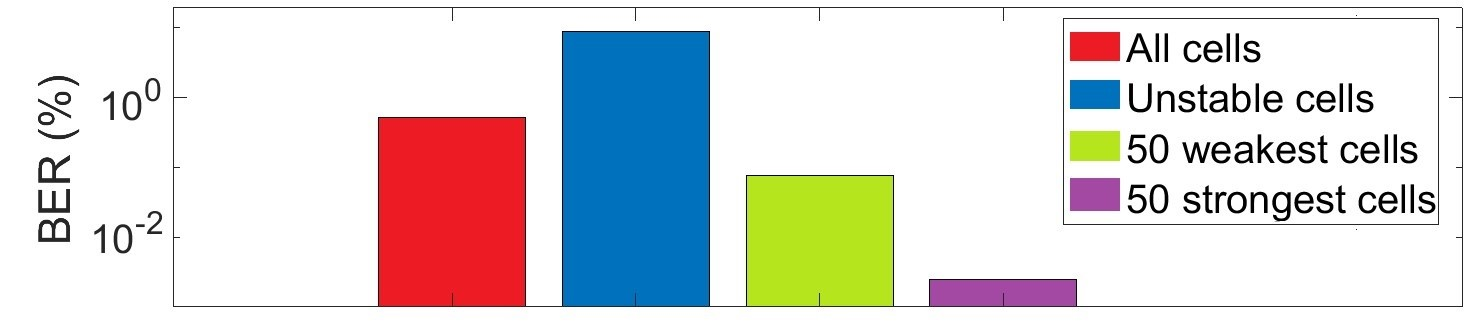
\includegraphics[width=10cm]{images/histBERSnW.jpg}
    \caption{Average BER of the five chips taking into account all cells, only unstable cells, the 50 weakest cells and the 50 strongest cells. }
    \label{fig:BERhistSnW}
\end{figure}
The BER results indicate that the cells labelled as unstable during the first step of the MTSV method are those with a larger instability, and that, by just applying the first part of the MTSV procedure and discarding these cells, the reliability of the PUF is largely increased. Once the unstable cells have been discarded, the remaining cells are classified  according to their DRV value, and the strongest ones are selected. Table \ref{tab:Nom_ave_BER} and Figure \ref{fig:BERhistSnW} show that this further improves the reliability of the PUF, since the 50 strongest cells according to their DRV have $\sim30$ times less power-up errors than the 50 weakest ones, and $\sim210$ times less power-up errors than when no classification is done and the whole array is considered.

As a final remark to highlight the strength of the cells selected by the MTSV method, a 0.0025\% BER means that, in average, the strongest cells yield an erroneous power-up only once out of 40,000 times. It becomes thus evident that a typical Multiple Evaluation test with some tens of power-ups, like those in \cite{Bhargava2012,Baturone2015}, would not be able to achieve such a selection. This is the reason for choosing a very high number of power-up evaluations to test the cells that were not discarded during the first part of the MTSV test.
In the following subsections, the capacity of the MTSV method to select strong cells in the presence of circuit aging and temperature and supply voltage variations will be evaluated. For this, the focus will be set on the strongest and weakest cells, since it has already been shown at nominal conditions that the cells labelled as unstable by the MTSV method are not suitable to be used in PUF identifiers.

\subsubsection{Resilience to circuit aging}
\label{ss:aging}

The next step was to evaluate the adequacy of the MTSV method to select aging-resilient cells. For this, the 100 selected cells (50 strongest and 50 weakest) of one of the chips (chip \#1) were stressed (i.e., aged in an accelerated manner) to reinforce their non-preferred value. It must be clarified that this does not aim at emulating a real-case operation scenario, since SRAMs will age in different manners depending on the application they are used for. Therefore, the goal of this test is to represent a worst-case of aging degradation, in which its impact systematically reduces the cell power-up strength. To achieve this, their preferred value was written on each cell, and then the supply voltage was raised to \SI{2.5}{V} during 10,000 s. As mentioned in chapter \ref{chap:3}, the BTI aging suffered by an SRAM cell that stores a given value (e.g., ‘0’) drives the preferred power-up value of that cell towards the opposite value (e.g., ‘1’) \cite{Bhargava2012}. This aging is $V_{GS}$-activated, and can be accelerated by increasing this voltage over its nominal value (1.2V for the technology used in this work). This is achieved by increasing the supply voltage of the cell. After this high voltage is removed, there are both a permanent and a recoverable component of degradation. For this reason, several measurements have been performed to investigate the resilience of the cells against degradation: one right after the stress ended, and three additional measurements 3 days, 10 days and 40 days later, to observe the evolution of the power-up behavior during the BTI recovery. The experiment performed right after the end of the stress consists of only 150 power-ups so that the recovery of the degradation throughout the test is not very significant. The other experiments, performed some days/weeks after the end of the stress, consist of 2,500 power-ups for each cell. The results obtained for each test were compared to the golden response obtained at nominal conditions for that chip before the stress was applied. The results for these experiments are collected in Table \ref{tab:aging_ave_BER}.

\begin{table}[H]
  \centering
  \caption{Average BER of the 50 strongest and 50 weakest cells of chip \#1 after accelerated aging}
  
  \vspace{5mm}
    \begin{tabular}{|c|c|c|c|c|}
    \hline
     Time after stress & Right after stress & 3 days & 10 days & 40 days \bigstrut\\
    \hline
    BER (\%) 50 strongest & 0 & 0 & 0.0016 & 0.0008 \bigstrut\\
    \hline
    BER (\%) 50 weakest & 28.1200 & 21.0424 & 19.2640 & 18.5720 \bigstrut\\
    \hline
    \end{tabular}%
  \label{tab:aging_ave_BER}%
\end{table}%

In this case, the difference in resilience against accelerated aging between the cells classified as strong and weak by the MTSV method is quite revealing. The 50 strongest cells according to that method remain unaffected by aging in terms of their power-up response, having a BER of 0 (which means that there was no power-up different to the one in the golden response) or very close to 0 in each experiment. On the other hand, the BER of the 50 weakest cells is much larger than the values obtained at nominal conditions before the stress was applied. Before the stress, this value for all chips was ~0.08\% (see Table \ref{tab:Nom_ave_BER}), while now it is ~28\% right after the stress, and it slowly recovers down to ~19\%. This large increase in BER for the cells classified as weakest by the MTSV method, while those classified as strong maintain a very low BER, indicates that the MTSV method has correctly selected the cells that are more resilient to circuit aging in terms of power-up response. Notice that, according to the Multiple Evaluation method, both sets of weakest and strongest cells had been labelled as equally strong, since they both had 0\% erroneous power-ups at nominal conditions. This demonstrates how the MTSV is able to foresee, before the cells have suffered any type of aging, which ones are going to be more robust against it, and therefore proves to be outstanding when selecting cells that are resilient to aging.



To gain insight into how the strength of the cells has changed after the stress, the DRV values measured 10 days after application of the stress are depicted in Figure \ref{fig:DRV_hist_stress}. It can be seen how, although the average DRV of the 50 strongest cells, and with it their strength, decreases slightly after the application of the stress, it is still much larger than the fresh DRV of the 50 weakest cells. This explains the fact that, even after the stress, the cells classified as strongest by the technique proposed in this work still have a strong tendency towards the same value when powered up. On the other hand, the case of the 50 cells classified as weakest is very different. Only 33 out of the 50 weakest cells remain stable after the stress, while the remaining 17 cells lost their tendency towards a given value and, therefore, no DRV could be assigned to them. For this reason, only those 33 weakest cells are shown in the histogram at the bottom of Figure \ref{fig:DRV_hist_stress}. As it can be seen in that histogram, there was also a decrease in their average DRV of a few milivolts.
To shed some light on the behavior of the recoverable component of the degradation, the BER value measured in each of the tests shown in Table \ref{tab:aging_ave_BER} is plotted against the time elapsed from the stress in Figure \ref{fig:BER_ev}. Interestingly enough, the expected logarithmic recovery of degradation at device level (i.e., of the transistors’ threshold voltage) \cite{Rangan2003}, translates into a logarithmic recovery of BER after the application of the stress.


\begin{figure}[H]
    \centering
    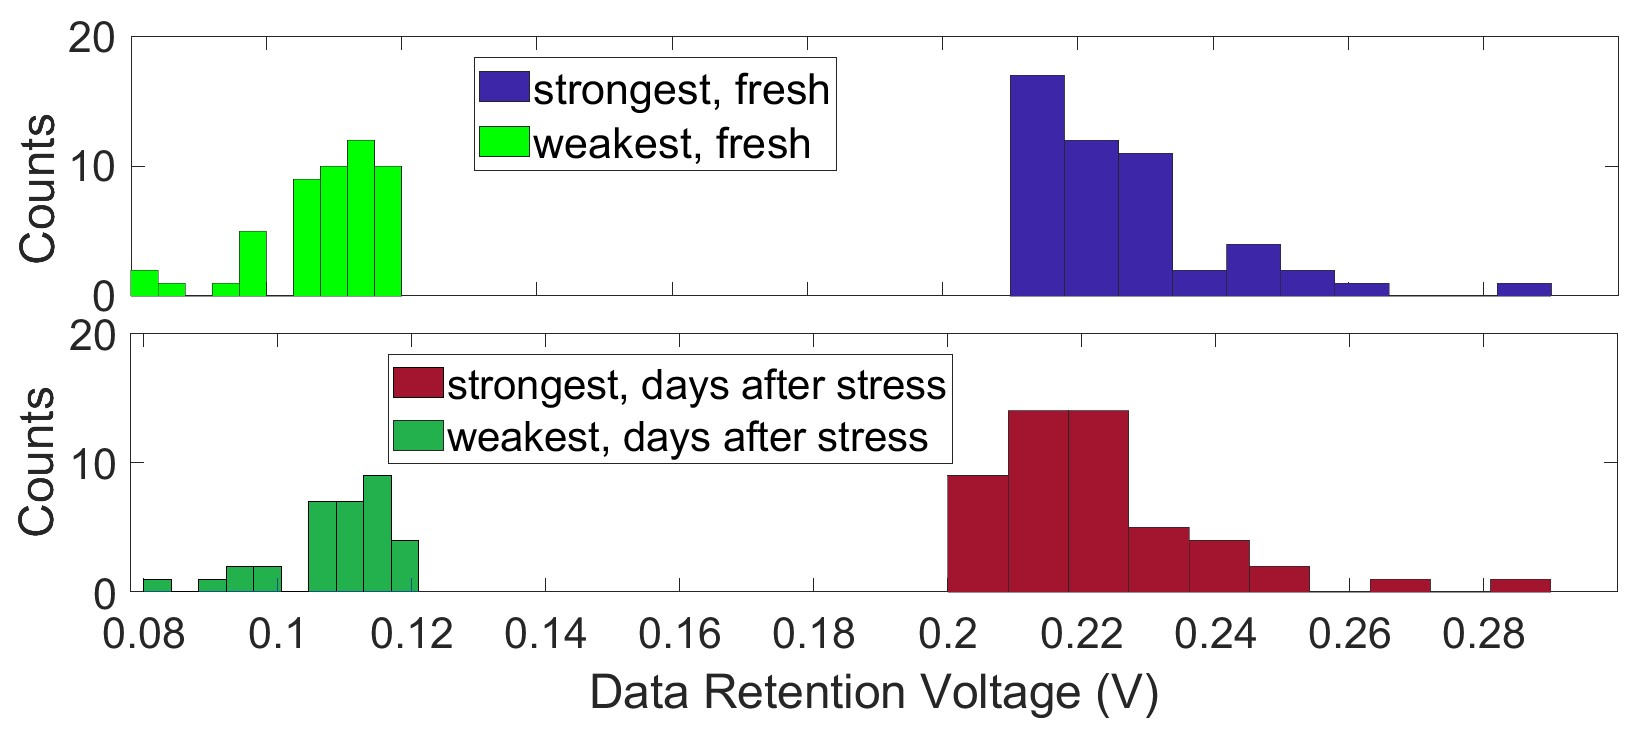
\includegraphics[width=10cm]{images/DRV_hist_stress.jpg}
    \caption{DRV value for the 50 strongest and 50 weakest cells measured before the stress (top), and 10 days after stress removal (bottom). }
    \label{fig:DRV_hist_stress}
\end{figure}

\begin{figure}[H]
    \centering
    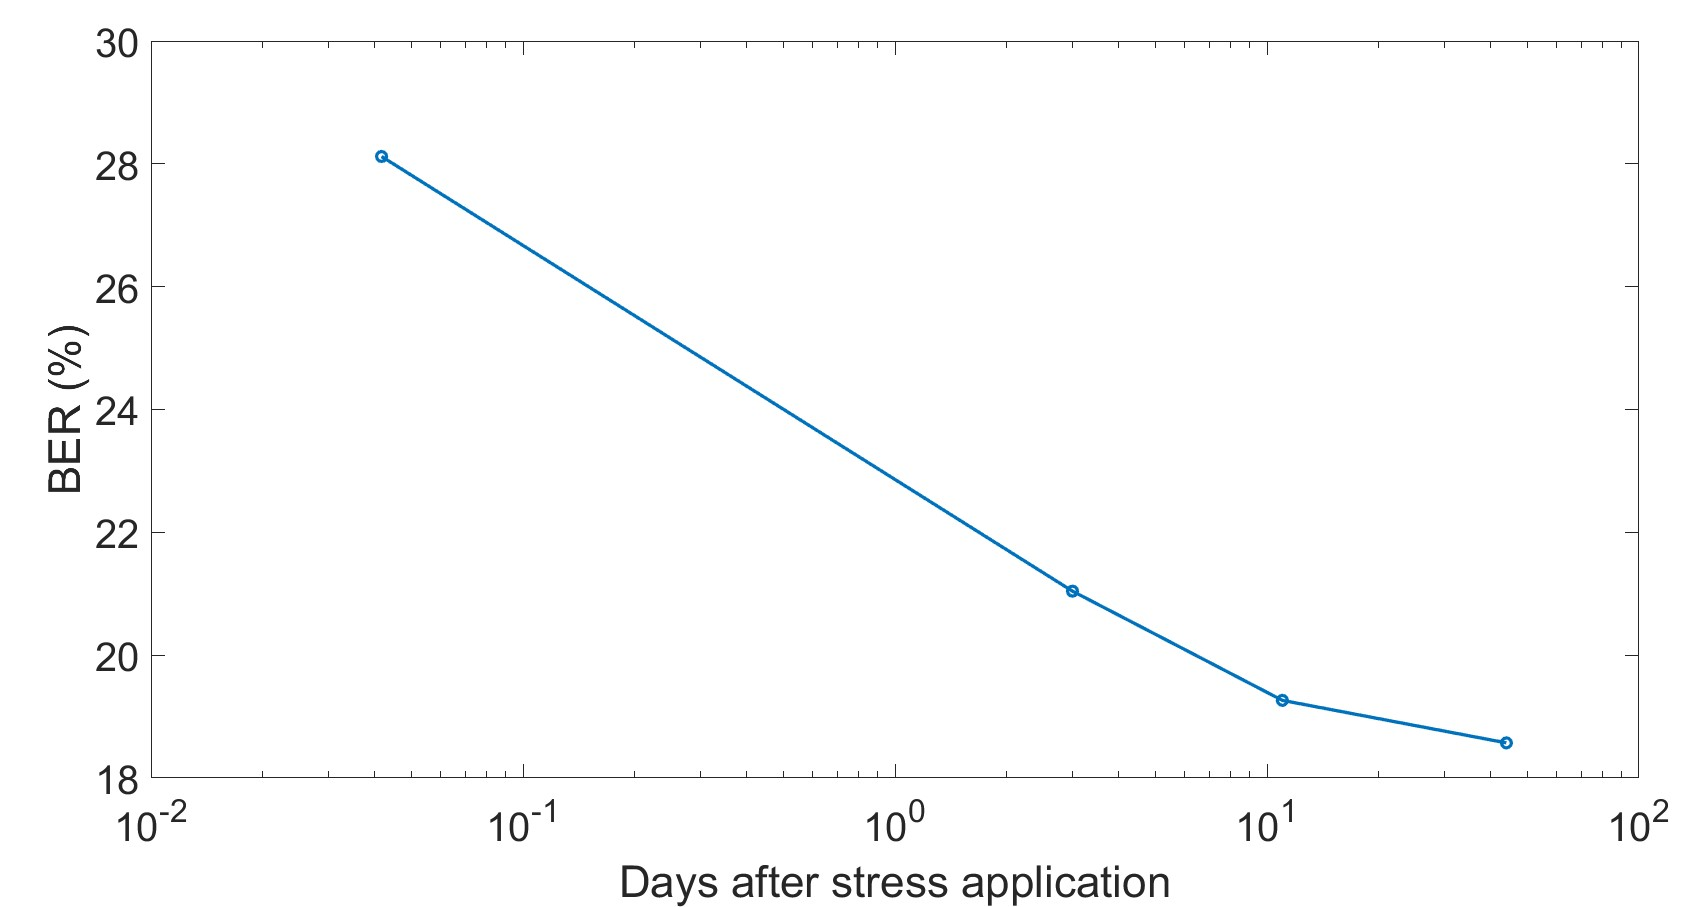
\includegraphics[width=10cm]{images/BER evolution.jpg}
    \caption{BER evolution for the 50 weakest cells of a chip with respect to the number of days since the application of the stress. }
    \label{fig:BER_ev}
\end{figure}

\subsubsection{Resilience to temperature variation}

To test the adequacy of the MTSV method under temperature variations, the 50 strongest and the 50 weakest cells of another chip (chip \#2) were selected under nominal conditions. Then, 2,500 power-ups were performed for each cell at $\SI{0}{\degree C}$, $\SI{10}{\degree C}$, $\SI{20}{\degree C}$, $\SI{30}{\degree C}$ and $\SI{40}{\degree C}$. The power-up response of the cells obtained under the different temperatures was evaluated using as a reference the golden response of that same chip obtained at room temperature, i.e., $\SI{25}{\degree C}$. The BER results are included in Table \ref{tab:temp_ave_BER}. 


Again, the 50 strongest cells according to the MTSV method prove to be very resilient against environmental variations, in this case against temperature variations ranging from $\SI{0}{\degree C}$ to $\SI{40}{\degree C}$. In fact, the worst BER obtained for the 50 strongest cells is 0.0024\%, which is even slightly lower than the average BER for the 50 strongest cells obtained at nominal conditions of temperature and supply voltage, which was 0.0025\%. The 0.0024\% BER obtained in the worst case for temperature variations translates into roughly 1 erroneous power-up out of every 42,000 evaluations. On the other hand, the performance of the cells classified as weakest by the MTSV method worsens when temperature variations are considered. For instance, the BER increases more than 10 times at both $\SI{0}{\degree C}$ and $\SI{40}{\degree C}$ compared to the one found at $\SI{20}{\degree C}$. The worst BER result for the 50 weakest cells is 1.7592\% at $\SI{0}{\degree C}$. This BER value corresponds to roughly 1 erroneous power-up out of every 57. This error rate is ~700 times larger than that of the strongest cells.
Similar to the circuit aging scenario discussed in the previous subsection, the results presented in Table \ref{tab:temp_ave_BER} prove that the MTSV method performed at nominal conditions has been able to correctly select the SRAM cells with a power-up behavior that better tolerate temperature variations. 


\begin{table}[H]
  \centering
  \caption{Average BER of the 50 strongest and 50 weakest cells of chip \#2 tested under temperature variations}
  \vspace{5mm}
    \begin{tabular}{|c|c|c|c|c|c|}
    \hline
     Temperature & $\SI{0}{\degree C}$ & $\SI{10}{\degree C}$ & $\SI{20}{\degree C}$ & $\SI{30}{\degree C}$ & $\SI{40}{\degree C}$ \bigstrut\\
    \hline
    BER (\%) 50 strongest & 0 & 0.0024 & 0.0008 & 0.0024 & 0.0008\bigstrut\\
    \hline
    BER (\%) 50 weakest & 1.7592 & 0.4080 & 0.1256 & 0.2288 & 1.2128 \bigstrut\\
    \hline
    \end{tabular}%
  \label{tab:temp_ave_BER}%
\end{table}%

\subsubsection{Resilience to Supply Voltage Variations}

The final test that has been performed was to test the adequacy of the MTSV method to select cells with a power-up response that is reproducible when supply voltage variations are introduced, since this type of fluctuations may be present in real application scenarios. For this, the 50 strongest and 50 weakest cells of one of the chips (chip \#2) according to the MTSV classification were powered-up 2,500 times each at room temperature and different supply voltages, i.e., raising their supply voltage from ground (\SI{0}{V}) to \SI{1.08}{V}, \SI{1.14}{V}, \SI{1.2}{V}, \SI{1.26}{V} and \SI{1.32}{V}. This corresponds to a range of the nominal voltage $1.2 \ \mathrm{V} \pm 10\%$. As in the previous tests, the results were compared to the golden response of the chip measured at nominal temperature and supply voltage conditions. The BER values obtained for this test are displayed in Table \ref{tab:vdd_ave_BER}. The worst BER value for the 50 strongest cells is obtained at $V_{DD} = \SI{1.2}{V}$ and is 0.0048\%, which corresponds roughly to one erroneous power-up out of every 21,000 power-ups. For the 50 weakest cells, the worst BER value is obtained at $V_{DD}$ = $\SI{1.32}{V}$ and is 0.204\%, 
equivalent to one erroneous power-up out of every 490, which corresponds to an increase in the error rate of ~70\% compared to the one obtained at nominal supply voltage conditions. As in the previous tests, these results make clear that the MTSV classification performed at nominal temperature and supply voltage conditions is able to select cells that will have an extremely reproducible power-up behavior even under supply voltage variations


\begin{table}[H]
  \centering
  \caption{Average BER of the 50 strongest and 50 weakest cells of chip \#2 tested under supply voltage variations}
  \vspace{5mm}
    \begin{tabular}{|c|c|c|c|c|c|}
    \hline
     Supply voltage & $\SI{1.08}{V}$ & $\SI{1.14}{V}$ & $\SI{1.20}{V}$ & $\SI{1.26}{V}$ & $\SI{1.32}{V}$ \bigstrut\\
    \hline
    BER (\%) 50 strongest & 0.0024 & 0.0016 & 0.0048 & 0.0008 & 0.0008\bigstrut\\
    \hline
    BER (\%) 50 weakest & 0.1160 & 0.1208 & 0.1216 & 0.1312 & 0.2040 \bigstrut\\
    \hline
    \end{tabular}%
  \label{tab:vdd_ave_BER}%
\end{table}%


